\documentclass[11pt,a4paper,german,notitlepage]{report}


%\usepackage[applemac]{inputenc} %Kommentierung entfernen,falls Mac
\usepackage[utf8]{inputenc} %Windows, Linux
%\usepackage[ansinew]{inputenc} %TeXnicCenter kann leider kein UTF-8

%Umlaute
%\usepackage[english]{babel}
\usepackage[ngerman]{babel}


\usepackage{natbib}
\bibliographystyle{humannat}


%einige Variablen definieren
\newcommand{\titelthema}{Thema der \\ Arbeit}
\newcommand{\authorname}{Vorname Name}
\newcommand{\authormail}{email@adresse.de}
\newcommand{\matrikelnr}{1234567}
\newcommand{\abgabedatum}{06. März 2012}
\newcommand{\betreuer}{ggf. Betreuer eintragen}
\newcommand{\arbeitstyp}{Bachelor-\textbackslash Masterarbeit}




% Standardschriftart
%\usepackage{times}
%\usepackage{garamond}

% Default-Schriften (\rmdefault Times, 
%\sfdefault Helvetica und \ttdefault Courier
%besser als \usepackage{times} da auch Mathematikschriften 
%berücksichtigt werden
\usepackage{mathptmx}  %Times
\usepackage[scaled=.92]{helvet}
%\usepackage{mathpazo} %Palatino
%\usepackage[scaled=.96]{berasans}
\usepackage{courier}

%Grafiken
\usepackage{graphicx}
\usepackage{subfigure} 

% Grafiken in einem Unterordner speichern
\graphicspath{{./images/}}


% Tabellen
%\usepackage{tabularx}

% Seitenränder
\usepackage[a4paper]{geometry}
\geometry{top=26mm, bottom=19mm, left=50mm, right=25mm, includefoot}

% Seitenränder auf Deckblatt
\usepackage[strict]{changepage}

%Querseiten mit korrekter Kopf-/Fußzeile
\usepackage{pdflscape}


%sauberer Blocksatz, optischer Randausgleich
\usepackage{microtype}


%1,5facher Zeilenabstand nur im Fließtext
\usepackage{setspace}
\onehalfspacing

%einfaches Anpassen von Kopf- und Fußzeilen 
\usepackage{fancyhdr}

\rhead{\small\thepage}
\lhead{\footnotesize\leftmark}
\chead{}
\rfoot{\footnotesize{\authorname, \the\year}}
\lfoot{\footnotesize{\arbeitstyp}}
\cfoot{}


% zusätzliche Sonderzeichen
%\usepackage{textcomp} 


% Mathematisches
%\usepackage{amssymb}
%\usepackage{amsmath} 
%\usepackage{amsfonts} 


% Code und Pseudocode
%\usepackage[ruled]{algorithm}
%\usepackage{algpseudocode}
%\usepackage[boxed]{algorithm}
%\usepackage{algpseudocode}

%Silbentrennung
\usepackage[T1]{fontenc}



% PDF options
\usepackage[hyperfootnotes=false, pdfpagelabels]{hyperref}
\urlstyle{rm}
\hypersetup{%
bookmarksopen={true},
%bookmarksopenlevel={2},
bookmarksnumbered=true,
pdfstartpage={1},
pdftitle={\arbeitstyp},
pdfsubject={\titelthema},
pdfauthor={\authorname},
pdfkeywords={},
pdfcreator={hyperref},
pdfproducer={LaTeX with hyperref},
pdffitwindow={false},
pdfpagelayout={SinglePage}
}


\usepackage{url}

\usepackage{color}
\usepackage{colortbl} %Für Listings
  \definecolor{dunkelgrau}{rgb}{0.7,0.7,0.7}
  \definecolor{hellgrau}{rgb}{0.9,0.9,0.9}

\usepackage{listing}
  \renewcommand{\listlistingname}{Quelltextverzeichnis}

\usepackage{listings}
  \lstset{numbers=left, numberstyle=\tiny, basicstyle=\scriptsize, backgroundcolor=\color{hellgrau}}
  \lstset{captionpos=b, aboveskip=15pt, belowskip=8pt, showstringspaces=false}
  \lstset{literate=%
  	{Ö}{{\"O}}1
	{Ä}{{\"A}}1
	{Ü}{{\"U}}1
	{ß}{{\ss}}1
	{ü}{{\"u}}1
	{ä}{{\"a}}1
	{ö}{{\"o}}1
	{~}{{\textasciitilde}}1
  }



%Abkürzungsverzeichnis, nur verwendete Abkürzungen darstellen
\usepackage[printonlyused]{acronym}

%Anhang
\usepackage{appendix}


%Bild-, Tabellenuntschriften schöner formatieren
\usepackage[format=hang,margin=10pt,font=small,labelfont=bf]{caption}

%PDF einbinden
%\usepackage{pdfpages}
%\includepdf[pages=1-4]{Meindoku.pdf}


%Euro 
%\usepackage{eurosym} 
% das Euro-Zeichen kann so eingefügt werden: \euro{}

%Lorem ipsum Auto-Text um Format zu zeigen
\usepackage{blindtext}


% Trennlinie unter der Kopfzeile
\renewcommand{\plainheadrulewidth}{0.4pt}


% Abstand zwischen Absätzen
%\parskip 3pt

% kein Erstzeileneinzug
%\setlength{\parindent}{0em}

\author{
\authorname\\
\texttt{\authormail}
}

\begin{document}
%
%%%%%%%%%%%%%%%%%%%%%%%%%%%%%%%%%%%%%%%%%%%%%%%%%%%%%%%%%	
%
\pagenumbering{roman}


\phantomsection
%\addcontentsline{toc}{chapter}{Deckblatt}
\pdfbookmark[0]{Deckblatt}{Deckblatt}
\label{Deckblatt}

% Eidesstattliche Erklärung notwendig
%
%%%%%%%%%%%%%%%%%%%%%%%%%%%%%%%%%%%%%%%%%%%%%%%%%%%%%%%%%%%
%
% Deckblatt
%

\thispagestyle{empty}
\begin{titlepage}

%Seite zentrieren
\begin{adjustwidth}{-2cm}{}


\renewcommand{\thepage}{}

\begin{center}

\large{Universität Regensburg\\}

\large{Fakultät für Wirtschaftswissenschaften\\}

\large{\mbox{Professur für Wirtschaftsinformatik - Prof. Dr. Guido Schryen}}

\vspace*{5mm}

\Large{\textbf{\titelthema}}

\vspace*{5mm}

\includegraphics[width=0.55\textwidth]{uni_logo.JPG}
\vspace*{4mm}

\Large{Bachelorarbeit}

\vspace*{5mm}


\end{center}
\begin{center}
Zur Erlangung des akademischen Grades "`Bachelor of Science (B.Sc.)"' im Studiengang\\
Wirtschaftsinformatik an der Fakultät für Wirtschaftswissenschaften der\\
Universität Regensburg.\\


\vspace*{5mm}

\Large{Eingereicht bei: Prof. Dr. Guido Schryen\\}

% \Large{Betreuung: \betreuer\\}

\end{center}

\vfill

\begin{center}
\large{Eingereicht am \abgabedatum\\}
\end{center}
\vspace*{0.6cm}
\begin{flushleft}
Eingereicht von:\\
\vspace*{7pt}
\authorname\\
Adresse\\
PLZ Ort\\
E-Mail Adresse: \authormail\\
Matrikelnummer: \matrikelnr\\




\end{flushleft}

\end{adjustwidth}

\end{titlepage}

\newpage

%%%%%%%%%%%%%%%%%%%%%%%%%%%%%%%%%%%%%%%%%%%%%%%%%%%%%%%%%
%%% Ende Deckblatt

%
%%%%%%%%%%%%%%%%%%%%%%%%%%%%%%%%%%%%%%%%%%%%%%%%%%%%%%%%%%%
%
% Deckblatt
%

\thispagestyle{empty}
\begin{titlepage}


%Seite zentrieren
\begin{adjustwidth}{-2cm}{}


\renewcommand{\thepage}{}

\begin{center}

\large{Universität Regensburg\\}

\large{Fakultät für Wirtschaftswissenschaften\\}

\large{\mbox{Professur für Wirtschaftsinformatik - Prof. Dr. Guido Schryen}}


\vspace*{5mm}

\Large{\textbf{\titelthema}}

\vspace*{5mm}

\includegraphics[width=0.55\textwidth]{uni_logo.JPG}
\vspace*{4mm}

\Large{Masterarbeit}

\vspace*{5mm}


\end{center}
\begin{center}
Zur Erlangung des akademischen Grades "`Master of Science (M.Sc.)"' im Studiengang\\
Wirtschaftsinformatik an der Fakultät für Wirtschaftswissenschaften der\\
Universität Regensburg.\\





\vspace*{5mm}

\Large{Eingereicht bei: Prof. Dr. Guido Schryen\\}

% \Large{Betreuung: \betreuer\\}

\end{center}

\vfill

\begin{center}
\large{Eingereicht am \abgabedatum\\}
\end{center}
\vspace*{0.6cm}
\begin{flushleft}
Eingereicht von:\\
\vspace*{7pt}
\authorname\\
Adresse\\
PLZ Ort\\
E-Mail Adresse: \authormail\\
Matrikelnummer: \matrikelnr\\




\end{flushleft}

\end{adjustwidth}

\end{titlepage}

\newpage

%%%%%%%%%%%%%%%%%%%%%%%%%%%%%%%%%%%%%%%%%%%%%%%%%%%%%%%%%
%%% Ende Deckblatt



% Eidesstattliche Erklärung _nicht_ notwendig
\include{DeckblattPraxisseminar}
\include{DeckblattProjektseminar}
%
%%%%%%%%%%%%%%%%%%%%%%%%%%%%%%%%%%%%%%%%%%%%%%%%%%%%%%%%%%%
%
% Deckblatt
%

\thispagestyle{empty}
\begin{titlepage}


%Seite zentrieren
\begin{adjustwidth}{-2cm}{}


\renewcommand{\thepage}{}

\begin{center}

\large{Universität Regensburg\\}

\large{Fakultät für Wirtschaftswissenschaften\\}

\large{\mbox{Professur für Wirtschaftsinformatik - Prof. Dr. Guido Schryen}}

\vspace*{10mm}

\Large{\textbf{\titelthema}}

\vspace*{15mm}

\includegraphics[width=0.55\textwidth]{uni_logo.JPG}
\vspace*{15mm}

\Large{Seminararbeit}

\vspace*{10mm}



\Large{Eingereicht bei: Prof. Dr. Guido Schryen\\}

% \Large{Betreuung: \betreuer\\}

\vspace*{5mm}

\large{Eingereicht am \abgabedatum\\}

\end{center}

\vfill

\begin{center}
\end{center}
\vspace*{6mm}
\begin{flushleft}
Eingereicht von:\\
\vspace*{7pt}
\authorname\\
E-Mail Adresse: \authormail\\
Matrikelnummer: \matrikelnr\\




\end{flushleft}

\end{adjustwidth}

\end{titlepage}

\newpage

%%%%%%%%%%%%%%%%%%%%%%%%%%%%%%%%%%%%%%%%%%%%%%%%%%%%%%%%%
%%% Ende Deckblatt



%Abstract einbinden
\phantomsection
%\addcontentsline{toc}{chapter}{Abstract}
\pdfbookmark[0]{Abstract}{abstract}
%
%%%%%%%%%%%%%%%%%%%%%%%%%%%%%%%%%%%%%%%%%%%%%%%%%%%%%%%%%%%
%
% Abstract
%

\thispagestyle{empty}

%Seite zentrieren
\begin{adjustwidth}{-2cm}{}

%Überschrift "Abstract" statt default "Zusammenfassung"
%\renewcommand{\abstractname}{Abstract}

%\begin{abstract}
%\label{abstract}
%Your abstract goes here...

%\blindtext

%\blindtext


\begin{Huge}\textbf{
\newline
\newline
\newline
\newline
\newline %Achtung: hier keine Leerzeile einfügen
Abstract}\end{Huge} \\ \\

\blindtext

\blindtext





%\end{abstract}

\end{adjustwidth}

%%%%%%%%%%%%%%%%%%%%%%%%%%%%%%%%%%%%%%%%%%%%%%%%%%%%%%%%%
%%% Ende Abstract


%%%%%%%%%%%%%%%%%%%%%%%%%%%%%%%%%%%%%%%%%%%%%%%%%%%%%%%%%


\newpage

% Keine Kopf-/Fußzeile auf den ersten Seiten
\pagestyle{fancyplain}

% "Kapitel" aus Kopfzeile weglassen
\renewcommand{\chaptermark}[1]{\markboth{\uppercase{\thechapter.\ #1}}{}}
% Nummerierungen nur bis Gliederungsebene 3 (\subsubsection)
\setcounter{secnumdepth}{3}
% Nur Überschriften bis Gliederungsebene 3 (\subsubsection) ins Inhaltsverzeichnis
\setcounter{tocdepth}{3}
\setcounter{page}{1}
\newpage


%Inhaltsverzeichnis
  \phantomsection
%  \addcontentsline{toc}{chapter}{Inhaltsverzeichnis}
  \pdfbookmark[0]{Inhaltsverzeichnis}{Inhaltsverzeichnis}
  \label{Inhaltsverzeichnis}
  \tableofcontents
  \newpage
  
%Abbildungsverzeichnis
  \clearpage
  \phantomsection
  \addcontentsline{toc}{chapter}{Abbildungsverzeichnis}
  \listoffigures
  \newpage

%Tabellenverzeichnis
  \clearpage
  \phantomsection
  \addcontentsline{toc}{chapter}{Tabellenverzeichnis}
  \listoftables
  \newpage

%Verzeichnis der Codelistings
  \clearpage
  \phantomsection
  \addcontentsline{toc}{chapter}{Listings}
  \lstlistoflistings
  \newpage

%Abkürzungsverzeichnis
% nur verwendete Abkürzungen werden dargestellt
  \clearpage
  \phantomsection
  \chapter*{Abkürzungsverzeichnis}
  \markboth{\uppercase{Abkürzungsverzeichnis}}{}
   \addcontentsline{toc}{chapter}{Abkürzungsverzeichnis}
   \begin{acronym}[MMMMMMMMM]
   %Kompaktansicht, Zeilenabstand verringern
   \setlength{\itemsep}{-\parsep}
   %Abkürzung fett
   \renewcommand*{\acsfont}[1]{{\textbf{#1}}}
   %auch für Abkürzungen Serifenschrift verwenden
   \renewcommand{\aclabelfont}[1]{\normalfont{\normalsize{#1}}\hfill}
      \acro{Bsp.}{Beispiel}
      \acro{SaaS}{Software as a Service}
      \acro{XML}{Extensible Markup Language}
   \end{acronym}
  \newpage

%Verhinderung von "Schusterjungen" und "Hurenkinder"
  \clubpenalty=10000
  \widowpenalty=10000 
  \displaywidowpenalty = 10000
  \tolerance=500 %Zeilenumbruch



%%%%%%%%%%%%%%%%%%%%%%%%%%%%%%%%%%%%%%%%%%%%%%%%%%%%%%%%%%%%%%%%%%%%%%%%%%

% Nummerierung wieder bei 1 beginnen
\setcounter{page}{1}

\pagestyle{fancy}
\pagenumbering{arabic}



%%%%%%%%%%%%%%%%%%%%%%%%%%%%%%% Einleitung %%%%%%%%%%%%%%%%%%%%%%%%%%%%%%%

%%%%%%%%%%%%%%%%%%%%%%%%%%%%%%%%% Einleitung %%%%%%%%%%%%%%%%%%%%%%%%%%%%%%%%%

\chapter{Einleitung}
\label{chap:Einleitung}

Eine Einleitung sollte möglichst präzise die aktuelle Forschungsfrage abbilden und dem
Leser die Zielstellung der Arbeit präsentieren. Durch eine Einordnung in den Gesamtzusammenhang
(inhaltlich/ zeitlich) wird für den Leser eine kompakte Übersicht gestaltet.
Dabei soll vor allem die Motivation, die zur Ausarbeitung der Arbeit geführt hat, dargelegt
werden. Dadurch wird dem Leser sowohl die Relevanz der Forschungsfrage, als auch
ein Grundverständnis der Thematik nahegebracht. Die Verwendung eines Zitates in der
Einleitung kann dabei helfen, die Notwendigkeit bzw. den Zweck der Arbeit verständlich
zu machen.
Im letzten Absatz der Einleitung wird die Struktur der Arbeit beschrieben, sprich: Das jeweilige Vorgehen wird grob beschrieben, sodass der Leser einen Einblick in den Aufbau der Arbeit erhält und sich darüber im Klaren sein kann, was diesen auf den kommenden Seiten erwartet.


%%%%%%%%%%%%%%%%%%%%%%%%%%%%%%%%%%%%%%%%%%%%%%%%%%%%%%%%%%%%%%%%%%%%%%%%%%%%%%


%%%%%%%%%%%%%%%%%%%%%%%%%%%%%%% Hauptteil %%%%%%%%%%%%%%%%%%%%%%%%%%%%%%%%

%%%%%%%%%%%%%%%%%%%%%%%%%%%%%%%%% Hauptteil %%%%%%%%%%%%%%%%%%%%%%%%%%%%%%%%%%

\chapter{Hauptteil}
\label{chap:Hauptteil}


\section{Beispiele}
Dies  ist eine Referenz auf ein Paper \cite{Webster2002} bzw. auf die Arbeit von Webster und Watson \cite{Webster2002}. Die Verwaltung der Referenzen erfolgt in der Datei References.bib. Zur Bearbeitung der Referenzen kann beispielsweise das Programm JabRef\protect{\footnote{\url{http://www.jabref.org/}}} verwendet werden.

Besonders interessant ist auch die automatische Erstellung des Abkürzungsverzeichnisses. Zuerst wird die Abkürzung definiert um bei erstmaliger Verwendung im Abkürzungsverzeichnis zu erscheinen: \ac{Bsp.}, \ac{SaaS}

Referenzen auf Grafiken: \ref{fig:Fig1}, \ref{img:subFig2}, \ref{img:subFigs}

\begin{figure}
  \centering
  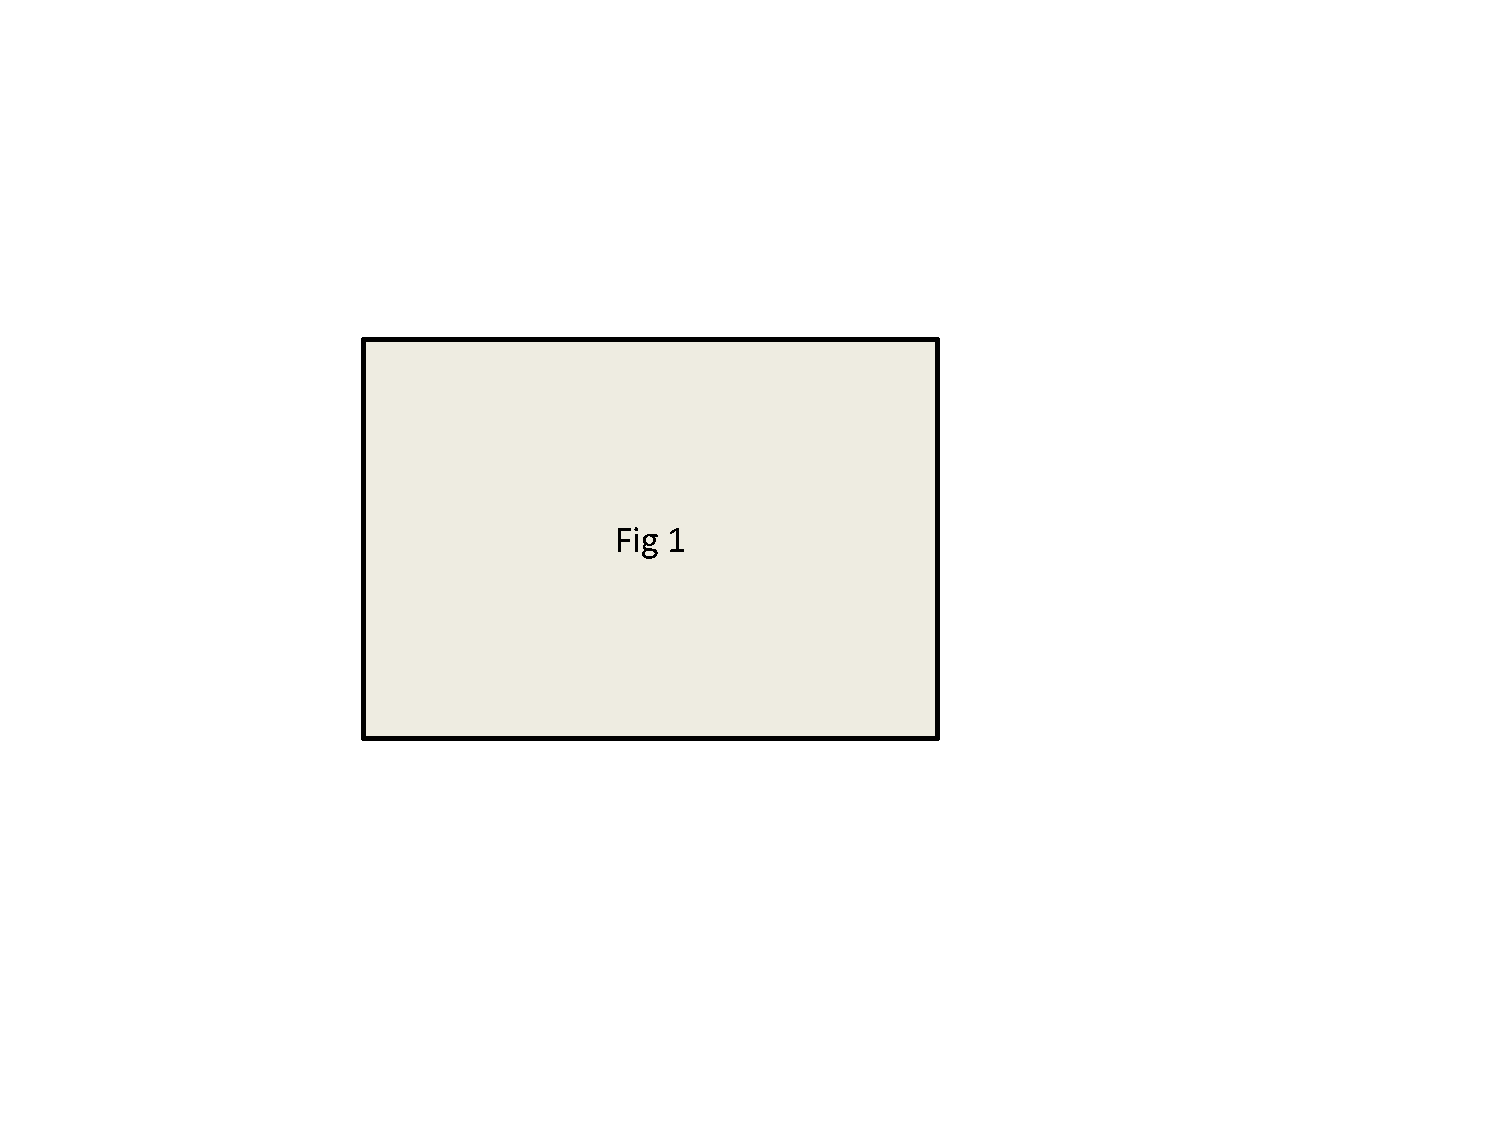
\includegraphics[width=0.95\textwidth]{Fig1.pdf}
  \caption{Beispielgrafik}
  \label{fig:Fig1}
\end{figure}


\begin{figure}
  \centering
  \subfigure[subfigure 1 \label{img:subFig1}]{\fbox{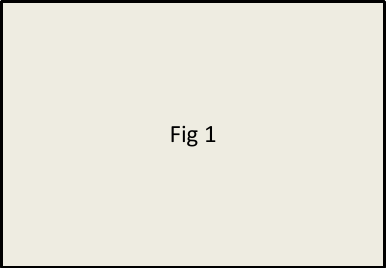
\includegraphics[width=0.45\textwidth]{Fig.png}}}\hfill
  \subfigure[subfigure 2\label{img:subFig2}]{\fbox{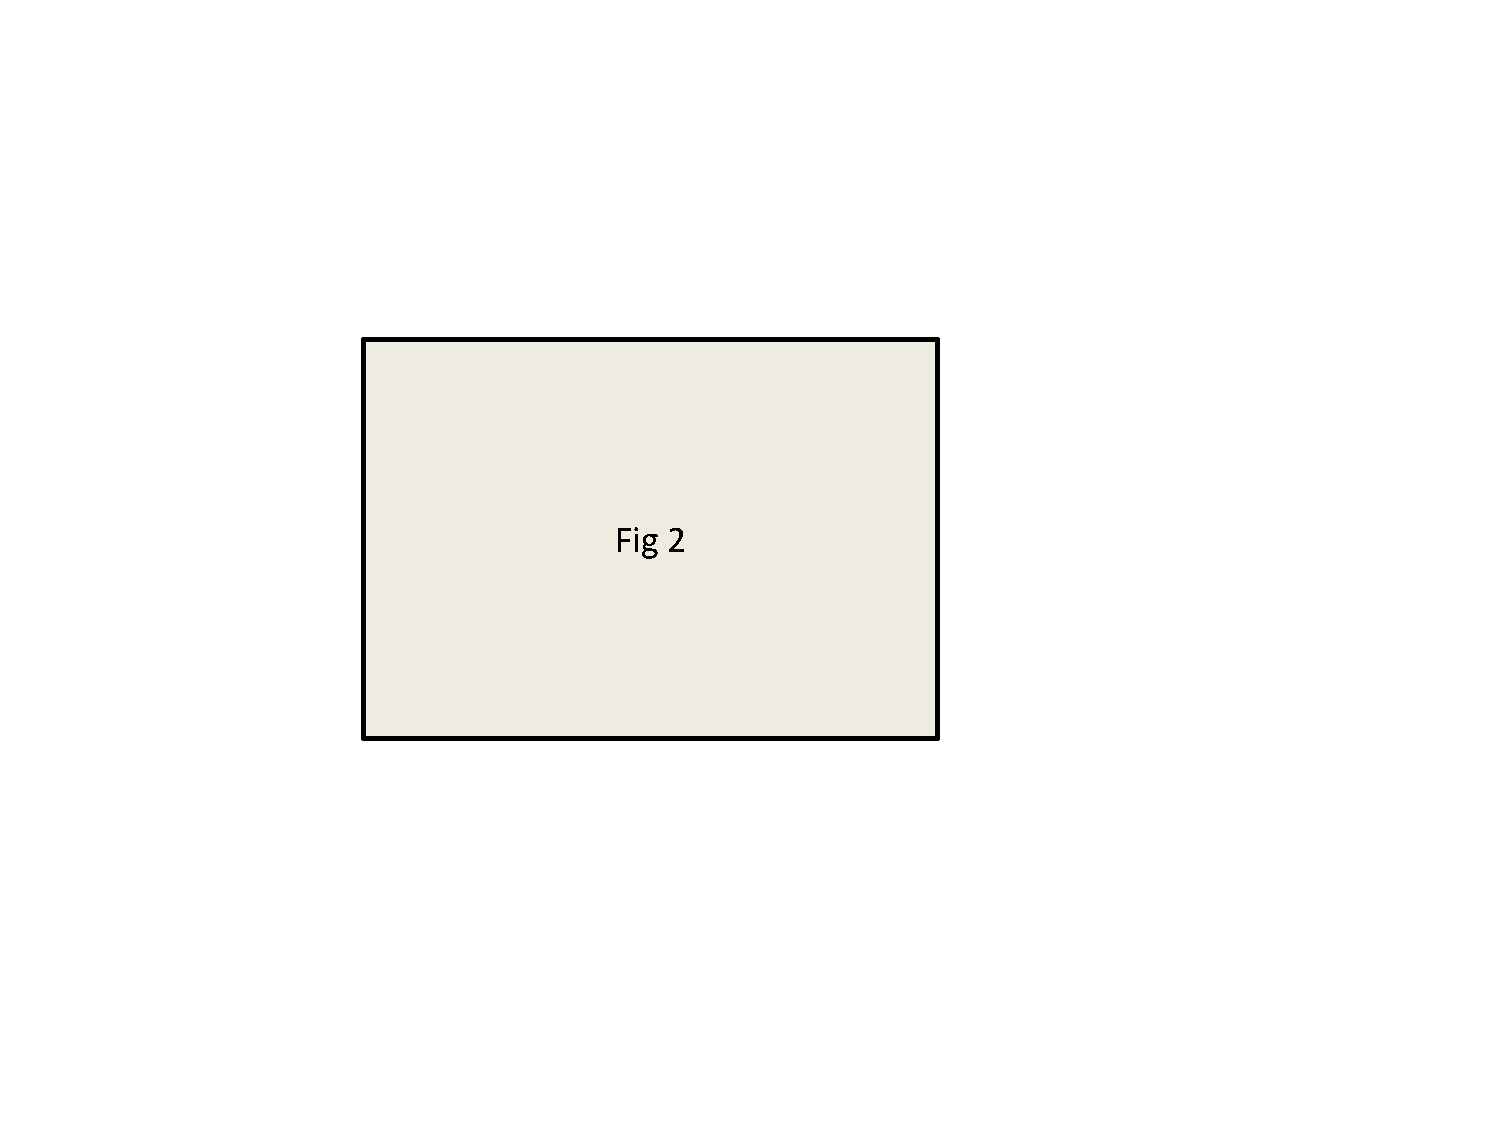
\includegraphics[width=0.45\textwidth]{Fig2.pdf}}}\hfill
  \caption{Beispiel subfigure}
  \label{img:subFigs}
\end{figure}



\lstset{language=JAVA, breaklines=true, tabsize=2}
\lstinputlisting[caption=HelloWorld,
label=lst:HelloWorld]{listings/HelloWorld.java}


%%%%%%%%%%%%%%%%%%%%%%%%%%%%%%%%%%%%%%%%%%%%%%%%%%%%%%%%%%%%%%%%%%%%%%%%%%%%%%


%%%%%%%%%%%%%%%%%%%%%%%%%%%%%%%% Schluss %%%%%%%%%%%%%%%%%%%%%%%%%%%%%%%%%

%%%%%%%%%%%%%%%%%%%%%%%%%%%%%%%%%% Schluss %%%%%%%%%%%%%%%%%%%%%%%%%%%%%%%%%%%

\chapter{Schluss}
\label{chap:Schluss}



%%%%%%%%%%%%%%%%%%%%%%%%%%%%%%%%%%%%%%%%%%%%%%%%%%%%%%%%%%%%%%%%%%%%%%%%%%%%%%


%%%%%%%%%%%%%%%%%%%%%%%%%%%%%%%%%%%%%%%%%%%%%%%%%%%%%%%%%%%%%%%%%%%%%%%%%%



%%%%%%%%%%%%%%%%%%%%%%%%% Literaturverzeichnis %%%%%%%%%%%%%%%%%%%%%%%%%%%

\renewcommand{\appendixpagename}{Anhang}

\newpage

\phantomsection
\addcontentsline{toc}{chapter}{Anhang}
\appendix
\appendixpage

%%\appendix
%%\phantomsection\appendixpagename{Anhang} 
% \renewcommand*
%%\appendixpage
%%\addappheadtotoc

\chapter{Erster Anhang}
\label{chap:anhang_1}

\chapter{Zweiter Anhang}
\label{chap:anhang_2}

\section{Anhang}
\label{sec:anhang_2_1}

\section{Anhang}
\label{sec:anhang_2_2}

\clearpage

%%%%%%%%%%%%%%%%%%%%%%%%% Literaturverzeichnis %%%%%%%%%%%%%%%%%%%%%%%%%%%
\phantomsection
\addcontentsline{toc}{chapter}{Literaturverzeichnis}
\bibliography{References}

\clearpage

%
%%%%%%%%%%%%%%%%%%%%%%%%%%%%%%%%%%%%%%%%%%%%%%%%%%%%%%%%%%%%%%%%%%%%%%%%%%
%% Eidesstattliche Erklärung %%%%
%
% nur bei Abschlussarbeiten!
%

\thispagestyle{empty}
\phantomsection
\label{erklaerung}
%\addcontentsline{toc}{chapter}{Erklärung}
\pdfbookmark[0]{Eidesstattliche Erklärung}{erklaerung}

\setlength{\parindent}{0em}

\markboth{\uppercase{Eidesstattliche Erklärung}}{}
\textbf{\large{Erklärung an Eides statt}}

\vspace*{20pt}
Hiermit versichere ich an Eides statt, dass ich die vorliegende Arbeit selbständig verfasst und keine anderen als die angegebenen Quellen und Hilfsmittel benutzt habe. Die aus fremden Quellen direkt oder indirekt übernommenen Gedanken sind als solche kenntlich gemacht. Die Arbeit wurde bisher in gleicher oder ähnlicher Form keiner anderen Prüfungsbehörde vorgelegt und auch nicht veröffentlicht.

\vspace*{65pt}


Regensburg, den \abgabedatum

\vspace*{60pt}


\authorname

Matrikelnummer \matrikelnr

\end{document}
